The motivation for this \textbf{boosting} method comes from the desire to better utilize the capability to perform a constant number of SVD calls on matrices as big as $[512\times 512]$ without slowing down UST considerably. As \textcolor{red}{XXX} tells us, the time complexity of SVD is \textcolor{red}{XXX}, so we treat 512 as the upper bound on the size of matrices we want to call SVD on. Recall the pipeline described in Figure ~\ref{fig:full-pipeline}. Pipeline level 1 and 2 use $E_5, E_4$ respectively to extract a 512-channels feature map representation of $I_c$ and $I_s$. This leads the WCT procedure to make two SVD calls on $[512\times 512]$ matrices, as described in ~\ref{sec:method_stylization}. We consider these calls \textit{efficient}. On the contrary, in levels 3,4,5, the feature maps the encoders extract have 256, 128 and 64 channels respectively. These calls are \textit{inefficient} since they call SVD on matrices of size lower than the upper bound.\\

The \textit{Boost} step is a procedure done after the WCT had output $f_{cs}$ and before image reconstruction took place, in levels of the pipeline where there are inefficient SVD calls, i.e. in architectures 1, 2 and 3.\\
At encoder-decoder architecture $j\in\{1,2,3\}$, let $x$ be the input content, $f_c = E_j(x)$ be the content features, of dimensions $[c \times h \times w]$, and $f_s = E_j(s)$ be the style image features, of dimensions $[c \times h' \times w']$. The number of channels $c$ is either 64, 128 or 256.
\begin{itemize}
	\item This step will synthetically create $f_c^b$ and $f_s^b$ of 512 channels, but with reduced height and width, such that the total number of entries in $f_c$ is the same as in $f_c^b$ and likewise for $f_s$ and $f_s^b$. Maintaining tensor sizes is important since many times regular UST is working close to the GPU memory limit also without boosting, so we wouldn't wish to create tensors much larger than we already handle. For architecture-1, $c=64$. Choose 8 rectangular regions of size $[c \times h/4 \times w/2]$ from $f_c$ and 8 rectangular regions of size $[c \times h'/4 \times w'/2]$ from $f_s$. The regions are to be stacked on the channel dimension to achieve $f_c^b$ of size $[8c \times h/4 \times w/2]$ and $f_s^b$ of size $[8c \times h'/4 \times w'/2]$. Notice that $8c=512$ as desired. Similarly for architecture-2, choose 4 regions while dividing both height and width by factor of 2. For architecture-3 choose 2 regions while dividing height by 2, width is not divided in this case. 
	
	\item This calls the WCT procedure on $f_c^b$ and $f_s^b$ to obtain $f_{cs}^b$. Since both $f_c^b$ and $f_s^b$ have 512 channels, the two SVD calls in the WCT decompose $[512\times 512]$ matrices.
	
	\item Next, $f_{cs}^b$ is split across the channel dimension, to invert the stacking operation done previously. Let these splits be $r_1^b, \dots r_d^b$ where $d\in\{2,4,8\}$ depending on the architecture. These splits are now being treated as boosted style transformed regions of $f_{cs}$. For architecture-1 we get 8 such regions, for arch-2 we get 4 and for arch-3 we get 2.
	
	\item Lastly, these regions are being blended with $f_{cs}$. Let $R_i$ be the indices slicing region $i$ from $f_c$, i.e. $f_c[R_i]$ is the $i$-th region, then:
	\begin{equation}
	f_{cs}[R_i] = (1-k)*f_{cs}[R_i] + k*r_i
	\end{equation}
	$k$ is a kernel the size of the regions $r_i$ that blends the edges in a way $f_{cs}[R_i]$ makes more effect close to the rectangular region borders while $r_i$ makes more effect in the interior. We a 2D raised cosine for this end. 
\end{itemize}

\begin{figure}[h!]
	\centering
	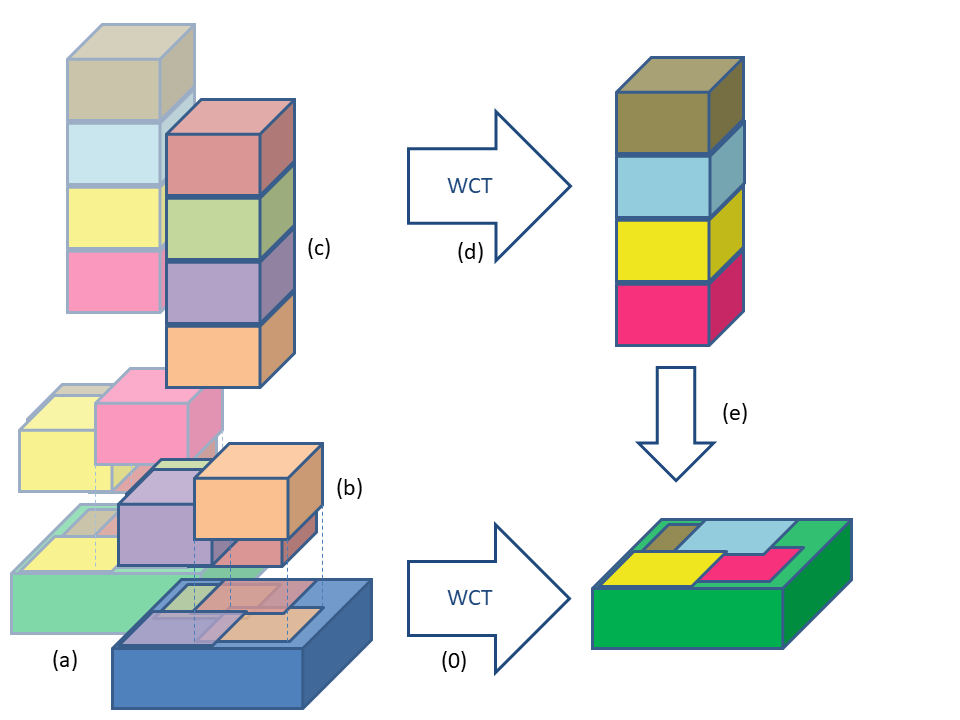
\includegraphics[width=0.5\linewidth]{boost_fig.png}
	\caption{Boost main steps. (0) is the ordinary WCT, (a) is regions selection, (b) is region slicing, in (c) the regions are stacked, in (d) WCT is performed on the stacked regions, finally in (e) the boosted regions are blended into $f_{cs}$.}
	\label{fig:boost}
\end{figure}

Before refining the boost method to its final form we had tried to replace the original WCT altogether in architectures 1,2 and 3, such that \textbf{only} efficient SVD calls are conducted. Doing so, regions were not chosen, instead, the features were perfectly divided into non overlapping sections. These were stacked, then came WCT and after which the sections were unstacked. The major drawback of that method is that these sections are treated as independent channels in the WCT, so clear border artifacts could be seen between them after the unstack and reconstruction operations.


